\section {Measurement Circuitry: Version 1}

\subsection {Overview}

This section will describe version 1 of the circuitry proposed to measure the parameters needed to analyze a capacitor. It will present analytical and empirical assessments of each circuit section where feasible and applicable.

\subsection {Protection}

This subsection will explain the protection circuitry used to isolate parts of the circuit from the high DC voltage in the event of a failure.

\subsection {(Dis)Charge Circuitry}

This subsection will explain the circuit used to (dis)charge the DUT and the circuit used to measure the current through the DUT.

The basic purpose of this section is to measure the charge/discharge curves of the DUT by stepping the input voltage and then measuring the current through the device over time.

\begin{figure}[ht!]
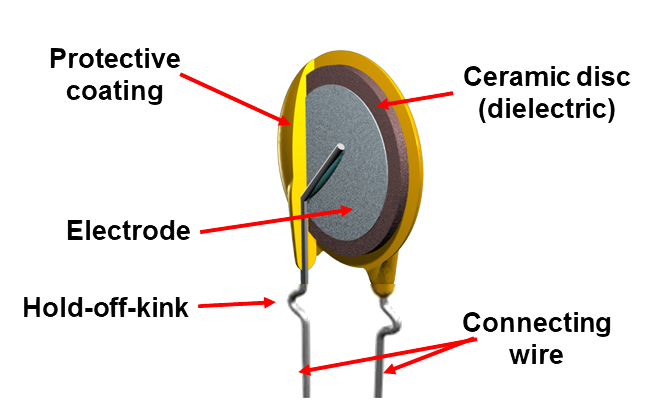
\includegraphics[keepaspectratio=true,scale=.5]{./figures/testImage.png}
\centering
\caption{(Dis)(Charge) Block Diagram}
\label{fig:cdlBlock}
\end{figure}


The block diagram depicted in Figure: \ref{cdlBlock} shows how this section will function. There are three basic modes:

Charging:
In this mode, the supply is set to the desired voltage and then stepped into the circuit with a relay. The input voltage sees a known resistor in series with the DUT to a virtual ground. The DUT will charge up to the input voltage according to its time constant. The virtual ground is made up of a transimpedance amplifier. It has the advantage of being able to measure on the low side of the DUT.

Discharging:
With the Charging side disconnected, a relay can connect the discharging circuitry to ground through a series resistor. The current measurement circuitry performs the same function, but with the opposite polarity measurement.

Leakage:
Once the DUT is charged to its full voltage, the steady state current can be measured over a much larger time period.

\subsubsection{Relay Control}
\begin{figure}
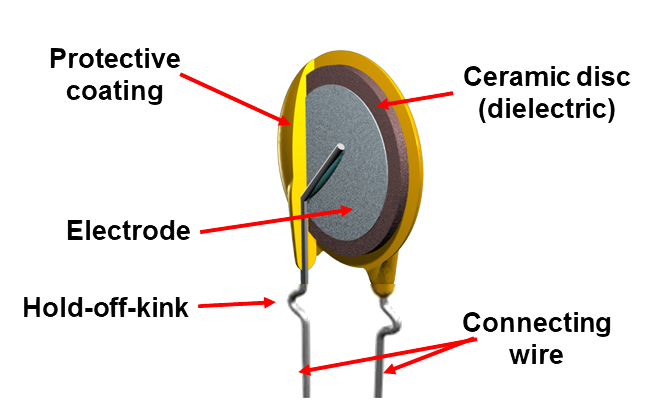
\includegraphics[keepaspectratio=true,scale=.5]{./figures/testImage.png}
\centering
%    \cite{capSite_df_vs_temp}
\caption{Relay Control Circuitry}
\label{cdlRelayCir_fig}
\end{figure}


Each relay is controlled with independent circuitry as shown in Figure: \ref{cdlRelayCir_fig}. The basic operation is that the input control signal (active high) switches either 5V or GND to the low side of the relay's coil. A ringback diode in series with a small valued resistor is in place to limit the coil's inductive spike while switching. Additionally there is a resistor + LED to indicate when an individual relay is active.

\subsection {AC Signal Injection}

This subsection will cover the circuitry and supporting tech needed to inject an AC signal onto the DUT.

\subsection {Transformer}

This subsection describes the equations and operation of the transformer used to inject the AC signal ont the DUT.

\subsection {AC voltage Measurement}

This subsection describes the AC voltage amplitude and phase measurements. 

\subsection {Rise and Fall Times}

This subsection describes the circuitry used to mesaure the rise and fall times of the DUT.

